\phantomsection
\section*{Chapitre 2 : La gestion budg\'etaire au Minist\`ere de la Justice}
\addcontentsline{toc}{section}{Chapitre 2 : La gestion budg\'etaire au Minist\`ere de la Justice}

\bigskip

Pr\'evoir l'ex\'ecution budg\'etaire d'un minist\`ere suppose d'en ma\^{\i}triser le cadre. Ce chapitre d\'ecrit la structure du budget du Minist\`ere de la Justice, les r\`egles impos\'ees par la LOF~130-13, et le cycle de la d\'epense publique~\citep{Bouvier2020}. Il aboutit sur les difficult\'es concr\`etes de pr\'evision qui motivent le recours \`a l'intelligence artificielle.

%================================================================
\phantomsection
\subsection*{2.1 \quad Le budget du Minist\`ere}
\addcontentsline{toc}{subsection}{2.1 Le budget du Minist\`ere}
%================================================================

%----------------------------------------------------------------
\phantomsection
\subsubsection*{2.1.1 \quad Composantes du budget}
\addcontentsline{toc}{subsubsection}{2.1.1 Composantes du budget}
%----------------------------------------------------------------

Conform\'ement \`a l'article~12 de la LOF 130-13, le budget de tout minist\`ere s'articule autour de trois instruments compl\'ementaires (figure~\ref{fig:structure-budget})~:

\begin{itemize}
    \item Le \textbf{budget g\'en\'eral (BG)}~: instrument principal retra\c{c}ant l'ensemble des recettes et des d\'epenses de l'\'Etat, \`a l'exception de celles retrac\'ees dans les SEGMA et les CST. Il concentre la quasi-totalit\'e des cr\'edits du minist\`ere de la Justice, r\'epartis entre d\'epenses de fonctionnement (article~14) et d\'epenses d'investissement (article~17). C'est sur ce p\'erim\`etre que porte l'analyse pr\'edictive d\'evelopp\'ee dans ce m\'emoire.

    \item Les \textbf{services de l'\'Etat g\'er\'es de mani\`ere autonome (SEGMA)}~: services non dot\'es de la personnalit\'e morale dont l'activit\'e tend \`a produire des biens ou \`a rendre des services donnant lieu \`a r\'emun\'eration (article~21). Leurs ressources propres doivent repr\'esenter au moins 30\,\% des ressources autoris\'ees \`a compter de la troisi\`eme ann\'ee suivant leur cr\'eation, sous peine de suppression. L'insuffisance \'eventuelle est compens\'ee par des subventions du budget g\'en\'eral. Le minist\`ere de la Justice dispose d'un SEGMA~: le \textit{Centre de Publication et de Documentation Judiciaire de la Cour de Cassation}.

    \item Les \textbf{comptes sp\'eciaux du Tr\'esor (CST)}~: comptes retra\c{c}ant des op\'erations sp\'ecialis\'ees pour lesquelles un lien direct existe entre recette et d\'epense (article~25). Le minist\`ere dispose de deux comptes d'affectation sp\'eciale (CAS)~:
    \begin{itemize}
        \item Le \textit{Fonds sp\'ecial pour le soutien des juridictions}~: cr\'e\'e en 1993 sous le nom de \og{}Fonds sp\'ecial pour l'extension et la r\'enovation des juridictions\fg{}, il a connu plusieurs modifications (1998, 2004, 2011). Depuis 2011, il est aliment\'e par 56\,\% du produit des amendes et p\'enalit\'es (hors code de la route), 56\,\% des recettes de la taxe judiciaire et 28\,\% des amendes routi\`eres, auxquels s'ajoutent des contributions du budget g\'en\'eral. En 2014, ses cr\'edits d\'efinitifs ont atteint 1,94~MMDH \citep{CourDesComptes2016}.
        \item Le \textit{Fonds d'entraide familiale}~: destin\'e au soutien des femmes divorc\'ees dans le besoin.
    \end{itemize}
\end{itemize}

\begin{figure}[htbp]
    \centering
    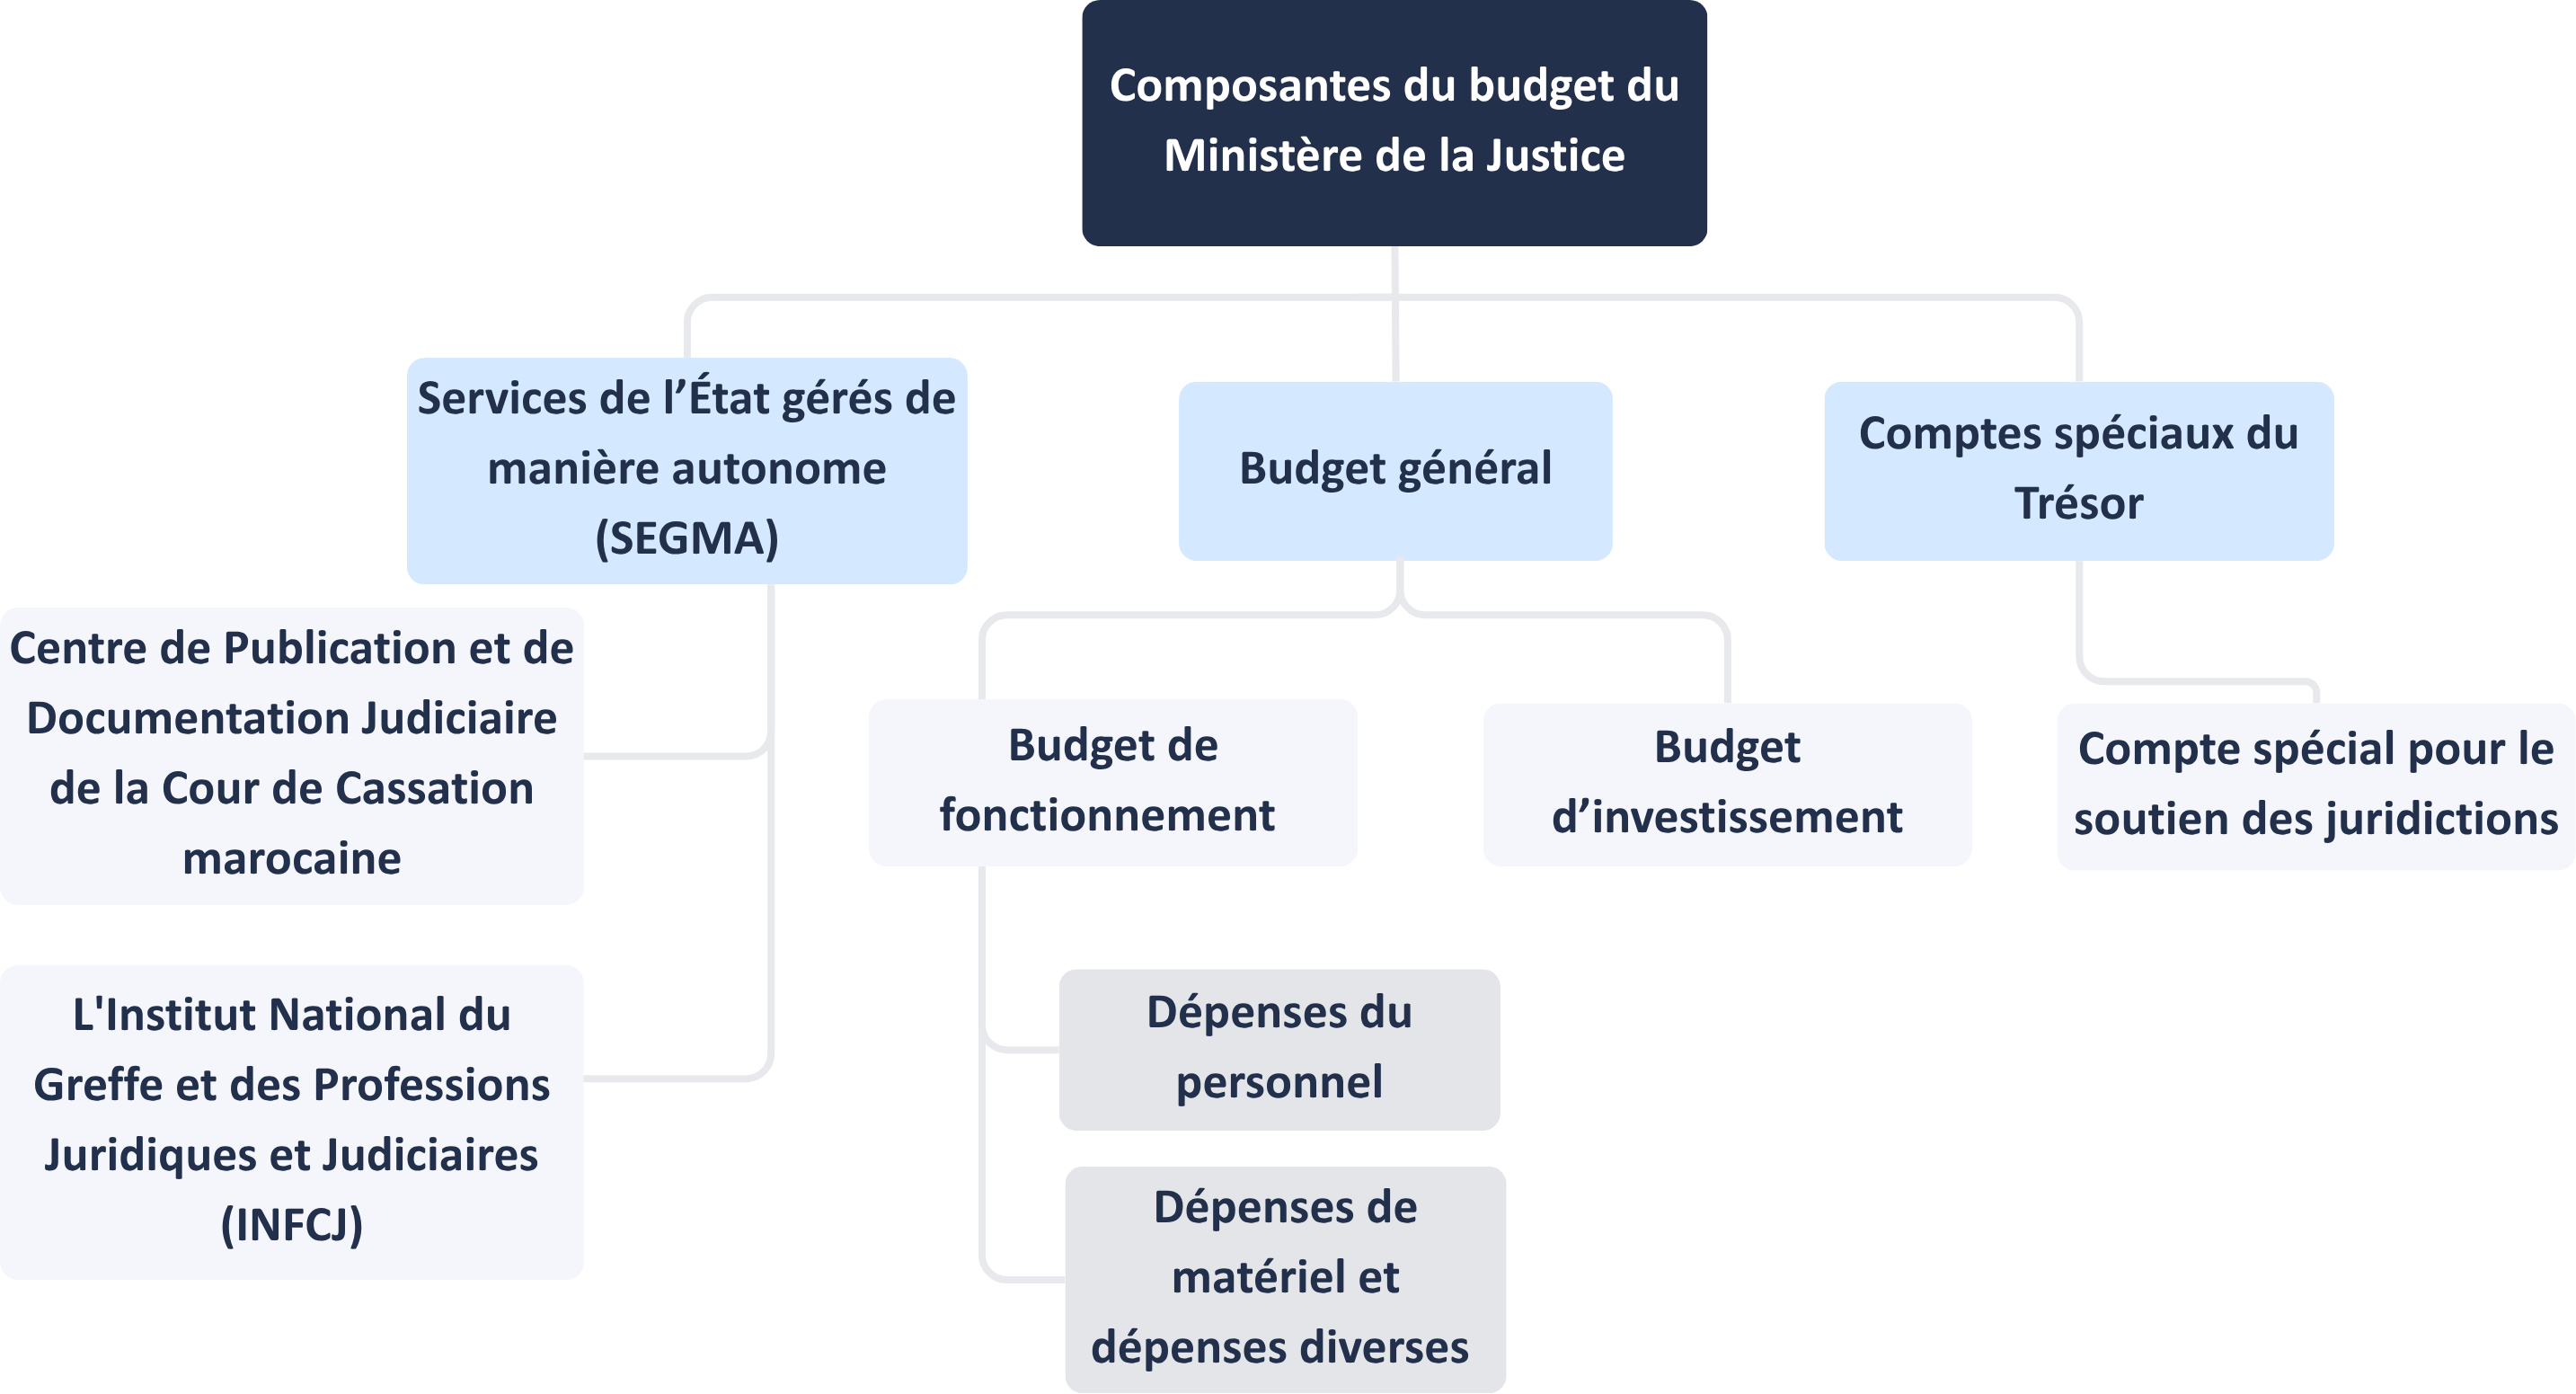
\includegraphics[width=\textwidth]{figures/structuredubudget.png}
    \caption{Composantes du budget du Minist\`ere de la Justice.}
    \label{fig:structure-budget}
\end{figure}

%----------------------------------------------------------------
\phantomsection
\subsubsection*{2.1.2 \quad D\'epenses et recettes du budget g\'en\'eral}
\addcontentsline{toc}{subsubsection}{2.1.2 D\'epenses et recettes du budget g\'en\'eral}
%----------------------------------------------------------------

Le budget g\'en\'eral concentrant la quasi-totalit\'e des cr\'edits du minist\`ere, c'est sur ce p\'erim\`etre que porte l'analyse pr\'edictive d\'evelopp\'ee dans ce m\'emoire. Il met en regard deux grandes masses~: les \textbf{d\'epenses}, qui couvrent les charges de fonctionnement et les d\'epenses d'investissement, et les \textbf{recettes}, qui correspondent aux ressources mobilis\'ees par l'\'Etat (imp\^ots et taxes, produit des amendes, r\'emun\'erations de services rendus, revenus du domaine de l'\'Etat et produit des emprunts) (LOF, article~11). Le budget du minist\`ere se structure autour de deux grandes cat\'egories de d\'epenses~:

\begin{itemize}
    \item Les \textbf{d\'epenses de fonctionnement}~: composante dominante et largement rigide. Elles comprennent la masse salariale (magistrats, greffiers, personnel p\'enitentiaire, administrateurs) et les d\'epenses mat\'erielles (alimentation des d\'etenus, carburant, maintenance, fournitures). La masse salariale repr\'esente historiquement plus de 70\,\% des cr\'edits de fonctionnement \citep{MJMaroc2023}.

    \item Les \textbf{d\'epenses d'investissement}~: consacr\'ees \`a la construction et \`a la r\'ehabilitation des palais de justice et des \'etablissements p\'enitentiaires, ainsi qu'\`a l'\'equipement informatique et logistique. Au cours de la p\'eriode 2010--2014, les cr\'edits d'investissement inscrits au budget g\'en\'eral ont atteint environ 3,26~MMDH (soit un montant annuel moyen de 651~MDH) \citep{CourDesComptes2016}. Ces cr\'edits pr\'esentent un profil d'ex\'ecution fortement concentr\'e sur le dernier trimestre de l'exercice.
\end{itemize}

Sur le plan des recettes propres, le minist\`ere g\'en\`ere des ressources li\'ees \`a l'activit\'e judiciaire~: le produit des amendes et p\'enalit\'es prononc\'ees par les juridictions, les droits de timbre judiciaires et la taxe judiciaire. La volatilit\'e de ces ressources constitue un facteur d'incertitude suppl\'ementaire dans la pr\'evision globale.

%================================================================
\phantomsection
\subsection*{2.2 \quad Le cadre juridique de la gestion budg\'etaire}
\addcontentsline{toc}{subsection}{2.2 Le cadre juridique de la gestion budg\'etaire}
%================================================================

%----------------------------------------------------------------
\phantomsection
\subsubsection*{2.2.1 \quad Les apports de la r\'eforme}
\addcontentsline{toc}{subsubsection}{2.2.1 Les apports de la r\'eforme}
%----------------------------------------------------------------

La loi organique n\textsuperscript{o}~130-13 relative \`a la loi de finances, promulgu\'ee en juin~2015 et mise en \oe{}uvre progressivement entre 2016 et 2020, constitue le socle r\'eformateur du cadre budg\'etaire contemporain. Conform\'ement \`a son article premier, elle \og{}d\'etermine, pour chaque ann\'ee budg\'etaire, la nature, le montant et l'affectation de l'ensemble des ressources et des charges de l'\'Etat, ainsi que l'\'equilibre budg\'etaire et financier qui en r\'esulte\fg{} \citep{MEF2015}.

La LOF a op\'er\'e une rupture fondamentale avec l'ancienne logique de \og{}budget de moyens\fg{} en instaurant une \og{}budg\'etisation par la performance\fg{}. L'objectif est, selon la formule du Guide de construction des programmes budg\'etaires, de \og{}faire mieux avec autant, voire moins de cr\'edits que les ann\'ees pr\'ec\'edentes\fg{} \citep{MEF2015b}. Cette nouvelle logique repose sur trois piliers~:

\begin{itemize}
    \item \textbf{La sinc\'erit\'e budg\'etaire} (article~10)~: les pr\'evisions doivent refl\'eter fid\`element les informations disponibles, sous peine d'observations de la Cour des Comptes ou de critiques parlementaires.

    \item \textbf{La programmation triennale} (article~5)~: chaque minist\`ere \'elabore une programmation budg\'etaire couvrant l'ann\'ee N et les deux ann\'ees suivantes (N+1 et N+2), actualis\'ee chaque ann\'ee.

    \item \textbf{La gestion ax\'ee sur les r\'esultats}~: chaque programme est associ\'e \`a des objectifs strat\'egiques et des indicateurs chiffr\'es, rendus publics dans les projets de performance (PdP) et les rapports annuels de performance (RAP) \citep{Khallouk2019}.
\end{itemize}

La LOF distingue trois cat\'egories de loi de finances (article~2)~: la \textbf{loi de finances de l'ann\'ee}, qui pr\'evoit et autorise l'ensemble des ressources et des charges pour un exercice donn\'e~; la \textbf{loi de finances rectificative}, qui modifie en cours d'exercice les dispositions de la loi initiale~; et la \textbf{loi de r\`eglement}, qui constate les r\'esultats financiers de chaque ann\'ee et approuve les \'ecarts entre les pr\'evisions et les r\'ealisations. C'est pr\'ecis\'ement la r\'eduction de ces \'ecarts que les mod\`eles pr\'edictifs d\'evelopp\'es dans ce m\'emoire visent \`a faciliter.

%----------------------------------------------------------------
\phantomsection
\subsubsection*{2.2.2 \quad La nomenclature budg\'etaire}
\addcontentsline{toc}{subsubsection}{2.2.2 La nomenclature budg\'etaire}
%----------------------------------------------------------------

La LOF a introduit une nouvelle architecture budg\'etaire organis\'ee en sept niveaux hi\'erarchiques. Les six premiers niveaux sont pr\'esent\'es dans les morasses budg\'etaires~; le septi\`eme est r\'eserv\'e \`a l'ex\'ecution \citep{MEF2015b}~:

\begin{enumerate}
    \item \textbf{Les titres} (article~38)~: Titre~I (fonctionnement), Titre~II (investissement), Titre~III (dette publique).
    \item \textbf{Les minist\`eres ou institutions}~: deuxi\`eme niveau de l'arborescence au sein de chaque titre.
    \item \textbf{Les chapitres}~: pour chaque minist\`ere, un chapitre personnel et un chapitre mat\'eriel et d\'epenses diverses (fonctionnement), et un chapitre investissement.
    \item \textbf{Les programmes} (article~39)~: unit\'e fondamentale de la budg\'etisation par la performance. Les cr\'edits d'un programme sont r\'epartis transversalement entre plusieurs chapitres.
    \item \textbf{Les r\'egions} (article~38)~: niveau g\'eographique permettant de suivre la r\'epartition territoriale des cr\'edits.
    \item \textbf{Les projets ou actions} (articles~38 et~40)~: d\'eclinaison op\'erationnelle du programme en activit\'es concr\`etes.
    \item \textbf{Les lignes budg\'etaires} (article~41)~: niveau d'ex\'ecution, renseignant la nature \'economique de la d\'epense. Ce niveau n'appara\^it pas dans les morasses publi\'ees avec le PLF~; il rel\`eve de la gestion interne du minist\`ere et n'est rendu public que dans le projet de loi de r\`eglement.
\end{enumerate}

\begin{figure}[htbp]
    \centering
    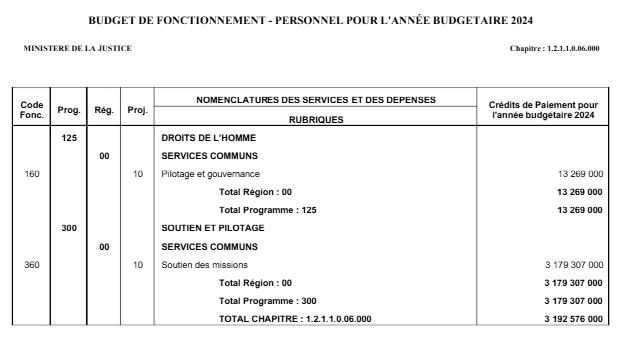
\includegraphics[width=\textwidth]{figures/morasse.png}
    \caption{Extrait de la morasse budg\'etaire du Minist\`ere de la Justice (exercice 2024).}
    \label{fig:morasse}
\end{figure}

%----------------------------------------------------------------
\phantomsection
\subsubsection*{2.2.3 \quad Les programmes budg\'etaires}
\addcontentsline{toc}{subsubsection}{2.2.3 Les programmes budg\'etaires}
%----------------------------------------------------------------

Le programme constitue le niveau structurant de la r\'eforme LOF. Conform\'ement \`a l'article~39, \og{}un programme est un ensemble coh\'erent de projets ou actions relevant d'un m\^eme d\'epartement minist\'eriel\ldots{} auquel sont associ\'es des objectifs d\'efinis en fonction des finalit\'es d'int\'er\^et g\'en\'eral ainsi que des indicateurs chiffr\'es permettant de mesurer les r\'esultats escompt\'es\fg{}.

Chaque programme se d\'efinit selon trois dimensions \citep{MEF2015b}~:

\begin{itemize}
    \item \textbf{Dimension budg\'etaire}~: le programme correspond \`a une enveloppe de cr\'edits consacr\'ee \`a une politique publique. C'est \`a ce niveau que s'op\`ere la \textit{fongibilit\'e asym\'etrique}~: les gestionnaires peuvent red\'eployer des cr\'edits \`a l'int\'erieur d'un m\^eme programme, \`a l'exception des cr\'edits de personnel \citep{MEF2015b}.

    \item \textbf{Dimension man\'ageriale}~: chaque programme est plac\'e sous la responsabilit\'e d'un responsable de programme, charg\'e de d\'efinir les objectifs, de piloter la mise en \oe{}uvre et de rendre compte des r\'esultats. Cette responsabilit\'e peut \^etre port\'ee par une personne ou par une \'equipe d\'edi\'ee, et s'inscrit au sommet d'une pyramide de pilotage couvrant les niveaux central et d\'econcentr\'e.

    \item \textbf{Dimension performance}~: les objectifs et indicateurs du programme sont pr\'esent\'es dans le \textbf{Projet de Performance (PdP)}, transmis au Parlement en accompagnement du PLF. La reddition de comptes s'effectue \`a travers le \textbf{Rapport Annuel de Performance (RAP)}, publi\'e avec le projet de loi de r\`eglement.
\end{itemize}

Le minist\`ere de la Justice dispose de quatre programmes budg\'etaires, dont la structure d\'etaill\'ee et l'\'evolution temporelle sont analys\'ees au chapitre~4.

%----------------------------------------------------------------
\phantomsection
\subsubsection*{2.2.4 \quad Le cycle de pr\'eparation du PLF}
\addcontentsline{toc}{subsubsection}{2.2.4 Le cycle de pr\'eparation du PLF}
%----------------------------------------------------------------

La pr\'eparation du Projet de Loi de Finances (PLF) suit un calendrier contraint fix\'e par la LOF (articles~47 et~48). Avant le~15~mars, le Chef du gouvernement invite par circulaire les minist\`eres \`a \'etablir leurs propositions de programmations budg\'etaires triennales assorties d'objectifs et d'indicateurs de performance. Avant le~15~avril, les minist\`eres transmettent leurs propositions au MEF. Les commissions de programmation et de performance les examinent avant le~15~mai. En juillet, le ministre des finances pr\'esente les grandes lignes du PLF au Conseil du gouvernement. En septembre--octobre, les propositions sont centralis\'ees et le PLF est d\'epos\'e au Parlement au plus tard le~20~octobre. La Chambre des repr\'esentants dispose de~30~jours pour se prononcer, suivis de~22~jours pour la Chambre des conseillers.

\begin{figure}[htbp]
    \centering
    \includegraphics[width=0.62\textwidth]{figures/phaseslof.png}
    \caption{Le cycle de pr\'eparation du Projet de Loi de Finances (PLF) au Maroc. \textit{Note~: le cycle d\'ebute en r\'ealit\'e d\`es mars par la circulaire du Chef du gouvernement aux minist\`eres (LOF, art.~47)~; la phase Avril--Mai correspond \`a la soumission formelle des propositions au MEF.}}
    \label{fig:cycle-plf}
\end{figure}

Ce calendrier contraint impose \`a la Direction du Budget de produire des pr\'evisions fiables dans des d\'elais courts~: les propositions budg\'etaires doivent \^etre finalis\'ees d\`es le mois de mars pour une ex\'ecution qui ne d\'ebutera qu'en janvier de l'ann\'ee suivante. C'est cette pression temporelle qui renforce l'int\'er\^et d'outils automatis\'es et robustes de projection.

%================================================================
\phantomsection
\subsection*{2.3 \quad L'ex\'ecution budg\'etaire}
\addcontentsline{toc}{subsection}{2.3 L'ex\'ecution budg\'etaire}
%================================================================

%----------------------------------------------------------------
\phantomsection
\subsubsection*{2.3.1 \quad Cr\'edits d'engagement et cr\'edits de paiement}
\addcontentsline{toc}{subsubsection}{2.3.1 Cr\'edits d'engagement et cr\'edits de paiement}
%----------------------------------------------------------------

L'article~18 de la LOF 130-13 organise le cycle d'ex\'ecution des d\'epenses d'investissement autour de deux instruments budg\'etaires distincts.

Le \textbf{cr\'edit d'engagement (CE)} repr\'esente la limite sup\'erieure des d\'epenses que les ordonnateurs sont autoris\'es \`a engager pour l'ex\'ecution des investissements pr\'evus. L'engagement constitue le premier acte de la d\'epense~: la d\'ecision par laquelle l'ordonnateur cr\'ee une obligation susceptible d'entra\^iner une charge pour l'\'Etat (signature d'un march\'e, commande de travaux). Les CE permettent des engagements pluriannuels tout en les rattachant \`a l'exercice de leur conclusion. Dans la pratique administrative, ce m\'ecanisme est couramment d\'esign\'e sous l'appellation \og{}autorisation d'engagement\fg{} (AE), terminologie emprunt\'ee au droit budg\'etaire fran\c{c}ais mais non retenue dans la LOF marocaine.

Le \textbf{cr\'edit de paiement (CP)} repr\'esente la limite sup\'erieure des d\'epenses pouvant \^etre ordonnanc\'ees et pay\'ees au cours d'un exercice pour honorer les engagements pass\'es. Les CP constituent la traduction financi\`ere annuelle des CE, qui peuvent s'\'etaler sur plusieurs ann\'ees pour des projets pluriannuels. La dissociation CE/CP g\'en\`ere des \textit{restes \`a payer} (RAP), \`a savoir des CE engag\'es non encore couverts par des CP, dont la gestion constitue l'un des d\'efis majeurs de la tr\'esorerie de l'\'Etat \citep{Bouvier2020}.

%----------------------------------------------------------------
\phantomsection
\subsubsection*{2.3.2 \quad Les quatre phases de la d\'epense}
\addcontentsline{toc}{subsubsection}{2.3.2 Les quatre phases de la d\'epense}
%----------------------------------------------------------------

Le cycle complet de la d\'epense publique comprend quatre phases r\'eglementaires, telles que d\'efinies par le D\'ecret royal n\textsuperscript{o}~330-66 portant R\`eglement G\'en\'eral de Comptabilit\'e Publique (RGCP) \citep{RGCP1967}. Ces phases s'organisent en deux volets distincts selon le principe fondamental de s\'eparation des fonctions d'ordonnateur et de comptable public.

\paragraph{La phase administrative~: du ressort de l'ordonnateur~:}

\begin{enumerate}
    \item \textbf{L'engagement}~: acte par lequel l'organisme public cr\'ee ou constate une obligation de nature \`a entra\^iner une charge. C'est la d\'ecision initiale qui pr\'el\`eve une partie des cr\'edits budg\'etaires en faveur d'un cr\'eancier~;
    \item \textbf{La liquidation}~: v\'erification de la r\'ealit\'e de la dette et arr\^et du montant exact de la d\'epense, au vu des pi\`eces justificatives attestant le service fait~;
    \item \textbf{L'ordonnancement}~: acte administratif donnant l'ordre de payer la dette. La liquidation \'etablit la dette~; l'ordonnancement lui conf\`ere un caract\`ere ex\'ecutoire.
\end{enumerate}

\paragraph{La phase comptable~: du ressort du comptable public (TGR)~:}

\begin{enumerate}
    \setcounter{enumi}{3}
    \item \textbf{Le paiement}~: acte par lequel l'organisme public se lib\`ere de sa dette. Le comptable public v\'erifie pr\'ealablement que le paiement est fait au v\'eritable cr\'eancier, sur un cr\'edit disponible et sur pr\'esentation de pi\`eces r\'eguli\`eres \'etablissant la r\'ealit\'e du service fait.
\end{enumerate}

\begin{figure}[htbp]
    \centering
    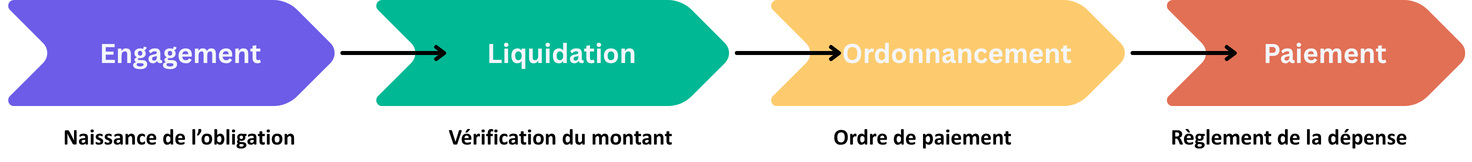
\includegraphics[width=0.72\textwidth]{figures/cycledepensespublique.png}
    \caption{Le cycle des d\'epenses publiques~: engagement, liquidation, ordonnancement et paiement.}
    \label{fig:cycle-depenses}
\end{figure}

Le cycle d'ex\'ecution au minist\`ere de la Justice est caract\'eris\'e par une \textbf{saisonnalit\'e marqu\'ee}~: les d\'epenses de fonctionnement suivent un rythme relativement r\'egulier, tandis que les d\'epenses d'investissement pr\'esentent un profil fortement concentr\'e sur le dernier trimestre, en raison des d\'elais de passation des march\'es publics et de la pression institutionnelle \`a consommer les cr\'edits avant la cl\^oture de l'exercice \citep{CourDesComptes2016}.

%----------------------------------------------------------------
\phantomsection
\subsubsection*{2.3.3 \quad Outils de suivi~: GID et morasse}
\addcontentsline{toc}{subsubsection}{2.3.3 Outils de suivi : GID et morasse}
%----------------------------------------------------------------

\paragraph{Le syst\`eme GID~:}

Le syst\`eme de \textbf{Gestion Int\'egr\'ee de la D\'epense (GID)}, d\'eploy\'e par la TGR depuis 2009, constitue le r\'ef\'erentiel central de l'ex\'ecution budg\'etaire dans l'ensemble des minist\`eres marocains. Inspir\'e d'exp\'eriences internationales (CHORUS en France, SIGFE au Chili, GIRES au Canada), il couvre toutes les phases de la d\'epense publique (gestion des cr\'edits, engagement, liquidation, ordonnancement et op\'erations de fin de gestion) et fournit une tra\c{c}abilit\'e compl\`ete de chaque op\'eration depuis l'ouverture des cr\'edits jusqu'au paiement par le comptable public.

La TGR met \`a disposition des ordonnateurs des \textbf{\'etats d'ex\'ecution budg\'etaire} indiquant, pour chaque programme, action et ligne budg\'etaire, les montants des cr\'edits ouverts, d\'el\'egu\'es, engag\'es, liquid\'es et ordonnanc\'es. Ces \'etats constituent la mati\`ere premi\`ere de notre analyse empirique.

\paragraph{La morasse budg\'etaire~:}

Il importe de distinguer ces \'etats d'ex\'ecution de la \textbf{morasse budg\'etaire} au sens strict de la LOF. Cette derni\`ere est un document annuel~: l'annexe d\'etaill\'ee au Projet de Loi de Finances (PLF) qui pr\'esente, programme par programme et chapitre par chapitre, la structure des cr\'edits demand\'es pour l'exercice \`a venir. Elle est publi\'ee une fois par an lors du d\'ep\^ot du PLF au Parlement. Notre analyse empirique s'appuie sur un jeu de donn\'ees reconstitu\'e \`a partir
de deux sources compl\'ementaires~: la morasse budg\'etaire annuelle (structure des
lignes, programmes, r\'egions et projets) et les rapports d'ex\'ecution trimestriels
publi\'es par la TGR (taux d'ex\'ecution agr\'eg\'es). Ce jeu de donn\'ees couvre
la p\'eriode 2021--2026 et est pr\'esent\'e en d\'etail au chapitre~4.

\paragraph{Le portail e-Budget~:}

Le portail \textbf{e-Budget} du MEF est utilis\'e en phase de programmation pour la saisie et la consolidation des propositions budg\'etaires lors des conf\'erences annuelles. Malgr\'e la disponibilit\'e du GID et de e-Budget, une part significative du travail d'analyse demeure r\'ealis\'ee \`a l'aide de tableurs, g\'en\'erant des risques d'erreurs et des silos d'information que notre projet contribue \`a corriger.

%================================================================
\phantomsection
\subsection*{2.4 \quad La pr\'evision budg\'etaire}
\addcontentsline{toc}{subsection}{2.4 La pr\'evision budg\'etaire}
%================================================================

%----------------------------------------------------------------
\phantomsection
\subsubsection*{2.4.1 \quad Sources de complexit\'e}
\addcontentsline{toc}{subsubsection}{2.4.1 Sources de complexit\'e}
%----------------------------------------------------------------

La LOF exige des pr\'evisions sinc\`eres, triennales et align\'ees sur des indicateurs de performance publics. Le D\'ecret n\textsuperscript{o}~2-22-580 du 3~mars~2023 renforce cette exigence en instituant dans chaque d\'epartement minist\'eriel un dispositif de contr\^ole de gestion charg\'e de \og{}mesurer les \'ecarts entre les r\'ealisations et les pr\'evisions et d'analyser les causes et les cons\'equences des \'eventuels \'ecarts\fg{} (article~7) \citep{DecretCDG2023}. Or la pratique budg\'etaire au minist\`ere de la Justice r\'ev\`ele des \'ecarts persistants entre pr\'evisions initiales et r\'ealisations effectives. Plusieurs fragilit\'es structurelles les expliquent~:

\textbf{La saisonnalit\'e des d\'epenses d'investissement~:} Les proc\'edures de passation des march\'es publics g\'en\`erent un cycle d'ex\'ecution concentr\'e sur le dernier trimestre~: les cr\'edits liquid\'es en novembre-d\'ecembre repr\'esentent une proportion disproportionn\'ee des r\'ealisations annuelles. Un contr\^ole de la Cour des Comptes a r\'ev\'el\'e que le taux de paiement des programmes d'investissement variait entre 23\,\% et 32\,\% sur la p\'eriode 2010--2014, tandis que les cr\'edits report\'es repr\'esentaient entre 42\,\% et 68\,\% des cr\'edits ouverts \citep{CourDesComptes2016}.

\textbf{La rigidit\'e de la masse salariale~:} Plus de 70\,\% des cr\'edits de fonctionnement sont pr\'eengag\'es par des charges de personnel dont l'\'evolution d\'epend de d\'ecisions administratives (recrutements, avancements, promotions) difficiles \`a projeter finement sur plusieurs ann\'ees.

\textbf{La dissociation CE/CP et les restes \`a payer~:} Les engagements pluriannuels cr\'eent une d\'ependance entre exercices~: les CP de l'ann\'ee N sont en partie d\'etermin\'es par les CE engag\'es en N-1 et N-2, ce que les m\'ethodes classiques de pr\'evision annuelle ignorent structurellement. Sur le Fonds sp\'ecial pour le soutien des juridictions, le taux d'engagement n'a oscill\'e qu'entre 28\,\% et 58\,\% des cr\'edits de paiement au cours de la m\^eme p\'eriode \citep{CourDesComptes2016}.

\textbf{La volatilit\'e des d\'epenses op\'erationnelles~:} Les d\'epenses hors masse salariale (alimentation des d\'etenus, carburant, maintenance) sont sensibles \`a des facteurs conjoncturels que l'extrapolation lin\'eaire ne peut int\'egrer.

\textbf{L'impact des chocs exog\`enes~:} La pand\'emie de COVID-19 (2020--2021) a illustr\'e les limites des mod\`eles fond\'es sur la continuit\'e des tendances~: suspension d'audiences, lib\'erations exceptionnelles de d\'etenus, gel de chantiers d'investissement.

%----------------------------------------------------------------
\phantomsection
\subsubsection*{2.4.2 \quad Limites des m\'ethodes actuelles}
\addcontentsline{toc}{subsubsection}{2.4.2 Limites des m\'ethodes actuelles}
%----------------------------------------------------------------

Les m\'ethodes de pr\'evision mobilis\'ees actuellement au minist\`ere s'appuient principalement sur l'extrapolation tendancielle et les projections lin\'eaires. Ces approches pr\'esentent plusieurs limites face \`a la complexit\'e des dynamiques budg\'etaires~:

L'incapacit\'e \`a capturer les \textbf{dynamiques non lin\'eaires}~: la concentration des d\'epenses d'investissement sur le dernier trimestre, l'accumulation des restes \`a payer, et les effets de seuil li\'es aux plafonds d'engagement ne peuvent \^etre repr\'esent\'es par des fonctions lin\'eaires.

Le \textbf{manque de r\'eactivit\'e}~: les m\'ethodes tendancielles int\`egrent lentement les nouvelles informations disponibles, alors que la pr\'eparation du PLF impose des actualisations fr\'equentes des pr\'evisions entre mars et octobre.

La \textbf{fragmentation de l'information}~: les donn\'ees utiles sont dispers\'ees entre plusieurs syst\`emes (GID, e-Budget, syst\`emes sectoriels de la DGAPR), et leur consolidation reste largement manuelle, co\^uteuse en temps et source d'erreurs.

L'absence de \textbf{m\'ecanismes d'incertitude explicites}~: les pr\'evisions produites sont ponctuelles, sans intervalles de confiance permettant aux d\'ecideurs d'appr\'ecier leur fiabilit\'e relative.

%----------------------------------------------------------------
\phantomsection
\subsubsection*{2.4.3 \quad Vers l'intelligence artificielle}
\addcontentsline{toc}{subsubsection}{2.4.3 Vers l'intelligence artificielle}
%----------------------------------------------------------------

Les insuffisances diagnostiqu\'ees dessinent un ensemble pr\'ecis de besoins m\'etiers et de contraintes op\'erationnelles pour des outils de pr\'evision alternatifs~: capacit\'e \`a exploiter l'historique disponible ligne par ligne~; r\'eactivit\'e face aux nouvelles informations~; et interpr\'etabilit\'e suffisante pour \^etre d\'efendable devant le MEF, le Parlement et la Cour des Comptes.

Les approches quantitatives modernes -- m\'ethodes statistiques classiques \citep{Hyndman2021} comme apprentissage automatique \citep{Russell2020} -- offrent des r\'eponses possibles \`a ces d\'efis, \`a condition d'\^etre s\'electionn\'ees en tenant compte de deux contraintes propres au contexte~: d'une part, l'historique exploitable est limit\'e \`a cinq exercices clos, ce qui exclut d'embl\'ee les mod\`eles plus riches en param\`etres, pour lesquels la litt\'erature recommande des effectifs d'un autre ordre de grandeur~; d'autre part, un mod\`ele qui pr\'edit mieux mais ne peut pas \^etre expliqu\'e -- ou pas ex\'ecut\'e dans l'environnement informatique du minist\`ere -- est inutile.

Le chapitre~3 d\'eveloppe les fondements th\'eoriques de ce double choix~: une famille de cinq mod\`eles parcimonieux (tendance lin\'eaire, moyenne historique, moyenne pond\'er\'ee, persistance, lissage exponentiel simple) avec s\'election ligne par ligne, et un dispositif de d\'etection d'anomalies combinant un score~$Z$ sur le taux d'engagement annuel et un algorithme \textit{Isolation Forest} dont les signaux sont crois\'es pour produire des niveaux de priorit\'e op\'erationnelle. Le chapitre~4 expose la mise en \oe{}uvre empirique de ce dispositif sur les fichiers \textit{SituationChap-AAAA.xls} du minist\`ere.
